\subsection{Temperatursensoren: PTC- und NTC-Thermistoren} % (fold)
\label{sub:Temperatursensoren: PTC- und NTC-Thermistoren}
\begin{frame}
    \frametitle{Thermistoren}
    \framesubtitle{}
    \begin{columns}[c]
        \column{0.6\textwidth}
            \begin{block}{Aufgabenstellung}
                 \begin{itemize}
                     \item Messen des Verhaltens bei
                        \begin{itemize}
                            \item Raumptemperatur
                            \item Erwärmung durch Reibung
                            \item Anschluss an Konstantstromquelle
                        \end{itemize}
                 \end{itemize}
            \end{block}
        \column{0.4\textwidth}
            \begin{figure}[H]
            \begin{center}
                   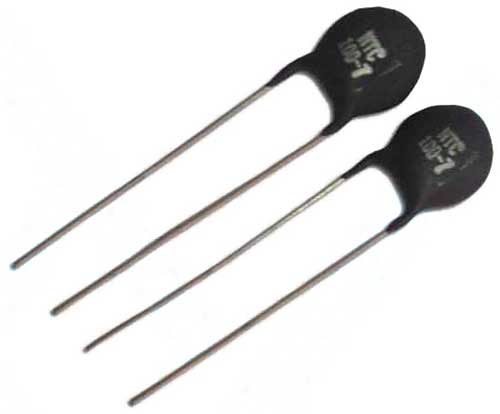
\includegraphics[scale=0.3]{./img/misc/thermistor.jpg}
            \end{center}
            \end{figure}
    \end{columns}
\end{frame}
\begin{frame}
    \frametitle{Bestimmung der Temperatur}
    \framesubtitle{}
    \begin{alertblock}{Problem:}
         \begin{itemize}
             \item PTCs nicht benannt
         \end{itemize}
    \end{alertblock}
    \pause
    \begin{center}
        \begin{tabular}{c|c}
            Thermistor & Widerstand \\
            \hline
            PTC: "langer" Streifen & $1.10k\Omega$\\
            PTC: "kurzer" Streifen & $0.11k\Omega$\\
            NTC: M87/G350 10k & $10.5k\Omega$
        \end{tabular}
    \end{center}
    \pause
    \begin{block}{}
        \begin{itemize}
            \item langer Streifen: PTC1000
            \item kurzer Streifen: PTC100
        \end{itemize}
    \end{block}
\end{frame}
\begin{frame}
    \frametitle{Bestimmung der Temperatur}
    \framesubtitle{}
    \begin{center}
        \begin{tabular}{c|c|c}
            Thermistor & $R_{DMM}/k\Omega$ & $T/^{\circ}C$\\
            \hline
            PTC1000 & $1.10$&$26$\\
            PTC100 & $0.11$&$26.85$ \\
            NTC: M87/G350 10k & $10.5$&$25$
        \end{tabular}
    \end{center}
\end{frame}
\begin{frame}
    \frametitle{Verhalten bei Reibung}
    \framesubtitle{}
        \begin{center}
            \begin{tabular}{c|c}
                Thermistor & Verhalten \\
                \hline
                PTC1000 & $R$ steigt\\
                PTC100 & $R$ steigt\\
                NTC: M87/G350 10k & $R$ sinkt
            \end{tabular}
        \end{center}
        \pause
        \begin{block}{Erklärung}
             \begin{itemize}
                 \item PTC sind Kaltleiter: schlechtere Leitung bei hohen Temperaturen
                 \item NTC sind Heißleiter: bessere Leitung bei hohen
                 Temperaturen
             \end{itemize}
        \end{block}
\end{frame}
\begin{frame}
    \frametitle{Anschluss an Konstantstromquelle}
    \framesubtitle{}
        \begin{center}
            \begin{tabular}{c|c|c|c|c}
                Thermistor & $U/V$ & $I/A$ & $R_{ber}/k\Omega$ & $T_{ber}/^{\circ}C$ \\
                \hline
                PTC1000 & $12.5$  & $0.010$ & $1.25$ &$64$\\
                PTC100  & $1.16$  & $0.010$ & $0.12$ &$41.85$\\
                NTC: M87/G350 10k & $16.8$ & $0.010$ & $1.68$ &$80$
            \end{tabular}
        \end{center}
        \begin{block}{}
            Konstantstrom erwärmt Widerstände $\rightarrow$ ungeeignet!
        \end{block}
        \begin{block}{Verhalten des NTCs:}
            \begin{itemize}
                \item 
                \begin{itemize}
                    \item U steigt auf $23V$
                    \item I steigt bis $10mA$
                    \item danach Abfall auf Messerte
                \end{itemize}
                \item Erklärung: Aufwärmphase in der NTC höheren Widerstand hat
            \end{itemize}
        \end{block}
\end{frame}
\begin{frame}
    \frametitle{Auswertung}
    \framesubtitle{}
    \begin{tabular}{c|c|c||c|c|c}
        Thermistor & $R_{DMM}/k\Omega$ & $T_{DMM}/^{\circ}C$ & $R_{ber}/\Omega$
        &$T_{ber}/^{\circ}C$\\
        \hline
        PTC1000 & $1.10$ & $26$ & 1.25 &$64$\\           
        PTC100  & $0.11$ & $26.85$ & 0.12 &$41.85$\\
        NTC: M87& $10.5$ & $25$ & 1.68 &$80$
    \end{tabular}
    \begin{block}{Messung des Widerstands}
         \begin{itemize}
             \item Konstantstromquelle
         \end{itemize}
    \end{block}
\end{frame}
% subsection Temperatursensoren: PTC- und NTC-Thermistoren (end)
